\section{\ivfsystem{} Implementation}

This section will go into the implementation details for the developed \ivfsystem{}.
Architecture, functions, data model, and the user interface design will be presented below.

The Rosemary architecture was fully reused, and domain-specific components for neuroimaging were removed, 
% for \ivfsystem{} implementation.
 as presented in section \ref{reuse-rosemary}. \silvia{ref to figure?}
On the level of code and structure, however, some changes were made to accommodate the \ivfsystem{} functionality.

Due to previously mentioned time restrictions not all functions that were discovered could be implemented.
A selection is made based on the programmers opinion what would be most profitable for a prototype system, considering that the prototype has to appeal to a wide variety of users, most importantly researchers and clinic management.
\silvia{before you said the priorities came from the brainstorm}
This selection is shown in figure \ref{fig:functions-workflow}: the implemented functions have a dashed border.

The system's critical functions have been implemented such as: user registration and management, data requests and acquisition.
To give the system eye-catchers and illustrate its potential value, the data audit has been implemented through so-called placeholders, \ie{} functions have pre-defined responses and do not work with the `live' data.
Also, different representation methods for data have been explored, for example: raw data, aggregated data, data in a graph.
This will be further explained in the user interface implementation details.

\paragraph{Functionality: back-end and front-end}
\silvia{misleading title}
The most notable changes to existing back-end code were in the security classes and data handling.
Rosemary already supports basic user management, where access to the system is provided based on the user account.
However the system needed to be extended with user roles for more fine-grained access control.
To execute this control the system requires these roles to be readable and actionable (\ie{} the system can act upon a specific role). \silvia{explain roles - here or somewhere?}
This is reflected in the {\tt Security} class which now supplies this information.

\silvia{i cannot understand this par. it is too abstract and uses "this" without being clear about what 'this" means:
Data handling had to be changed, as all the read methods in the {\tt Datum} class have been adapted to restrict access.
This makes for easy access of data from the front-end, the back-end filters the data and returns the restricted dataset.
The description of the data model implementation will explain this \silvia{what?} in detail.
An example of what this means in the front-end is shown in figure \ref{fig:dataset-example}.
}

\begin{figure}[ht]
	\centering
	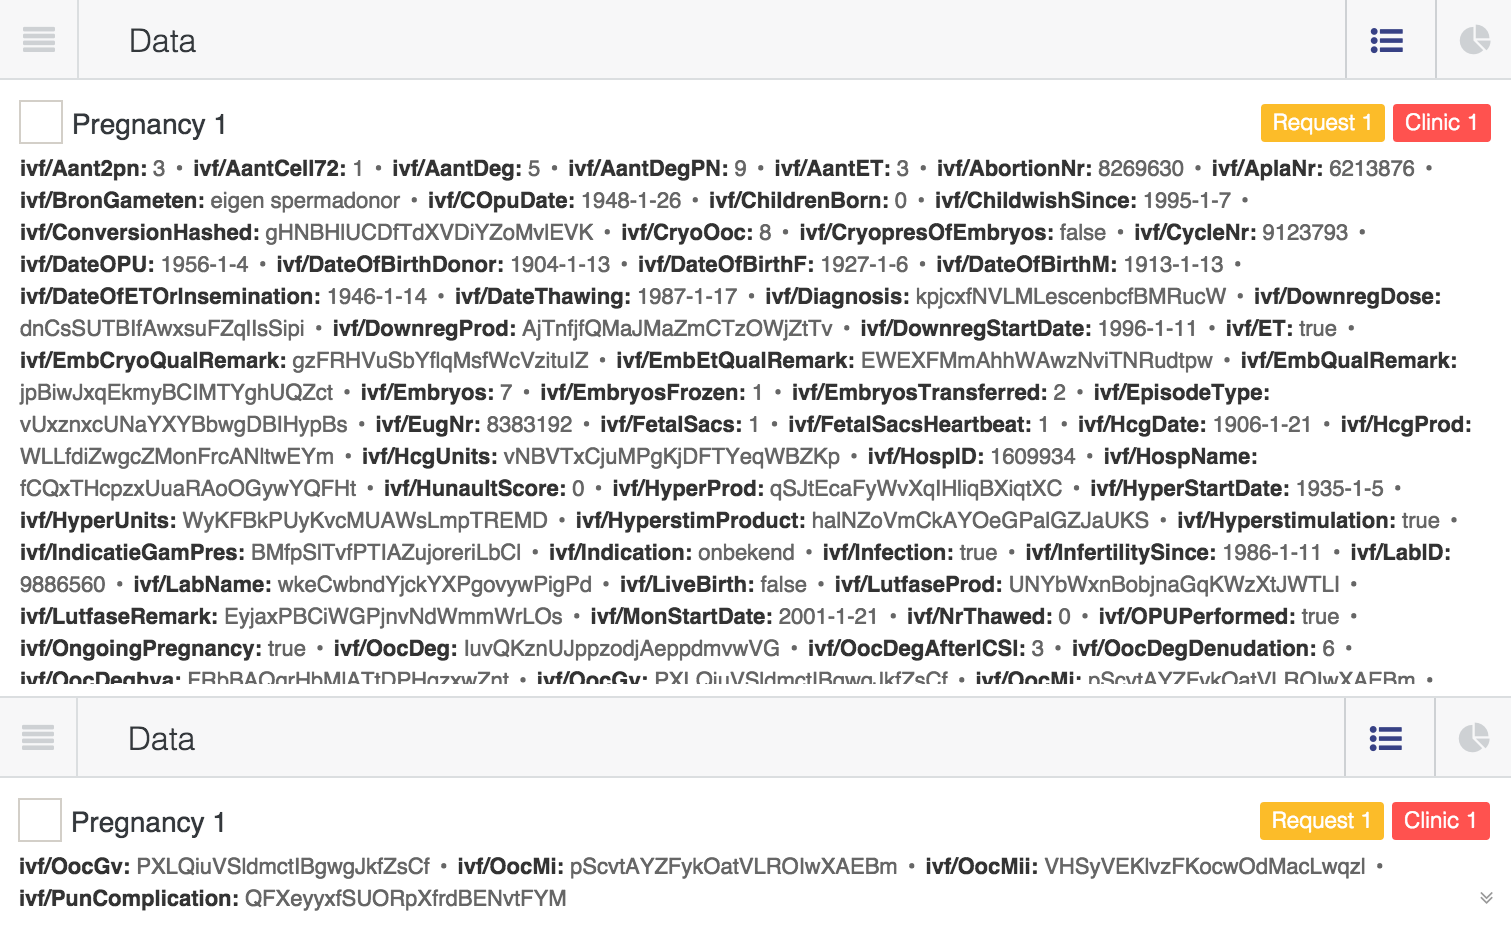
\includegraphics[width=1.0\linewidth]{images/datasets-example}
	\caption{
		Example of the full \projectdata{} (top) versus a restricted view (bottom).
		The restricted view shows exactly the same {\tt Datum} but only the accessible (four) headers are displayed.
	\silvia{put boxes around the two screenshots. which role is used at the bottom?}}
	\label{fig:dataset-example}
\end{figure}

\paragraph{Functionality: security}
\silvia{user management, roles, etc is part of security.}
Even though security considerations are a big part of the requirement analysis (see section \ref{security}), it does not show itself that clearly in the system implementation.
Most of the security measures were taken during the data gathering steps.
Because the decision was made to have a fixed dataset for the system a lot of the discussed security measures do not need to apply anymore as described in section \ref{security-summarisation-analysis}.

\silvia{too long par for something you did not do}
Provenance, as part of security, was not implemented either.
It would be very useful to show the strength of the \ivfsystem{}, data protection through provenance can be made highly visible and easy to understand for humans.
However, the goals to support the provenance functions and develop an interface on top of the data could not be reached within the time frame.

\silvia{i have the feeling that the presentation goes back and forth between model, arch, tech, and repeats explanations unnecessarily. cant you present everything related to data model in one place, then architecture, then function, etc? or in some other order?}

\begin{figure}[!b]
	\centering
	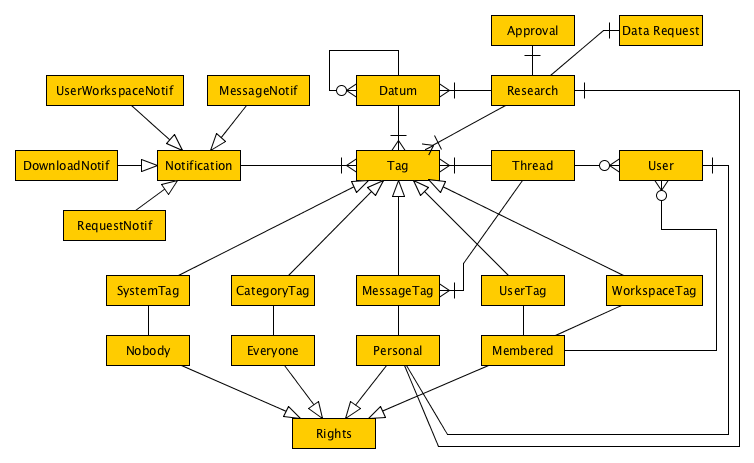
\includegraphics[width=0.8\linewidth]{images/datamodel-adapted}
	\caption{
		Rosemary data model as implemented. 
		Differences between the implemented \ivfsystem{} model and the original Rosemary model are shown in blue.
		Describes workspace, tagging, datum, notification, and research models.
	}
	\label{fig:implementation-rosemary-dm}
\end{figure}



\paragraph{The data model}
Unlike the architecture of Rosemary, the data model needed alterations to \silvia{integrate - is the gateway something different from rosemary?} with the \ivfsystem{}.
These can be divided into changes to already existing objects and additions of new objects.

One of the critical functionalities for the \ivfsystem{} is to support data requests on the \projectdata{}.
A request contains a limited set of data items (headers), the \projectdata{} contains all the available headers.
After a request has been approved the system creates a new subset which is accessible by the requesting researcher.
On the level of the data model this is achieved by tagging the {\tt Datum} objects with a {\tt WorkspaceTag}.
Only one {\tt User} has access to this tag and consequently dataset.

\silvia{i realize here that an example is missing to explain what you mean by data and metadata. put much earlier the explanation with examples of fields that can be requested}

In Rosemary tagging a {\tt Datum} exposes all the available data (and metadata) in this object.
A Request explicitly defines which data is needed. 
To support this the {\tt WorkspaceTag} object was extended with the set of headers \silvia{that should be accessible??}.
This refers back to the data handling as explained in section{xx}. The read methods for {\tt Datum} objects check the tag and filter the available data and metadata.

Also, the original Rosemary implementation does not differentiate between different \emph{types} of workspaces. 
The \ivfsystem{} has three types of  workspaces: the \emph{master} workspace containing the whole \projectdata{}, clinic workspaces containing data specific to a clinic, and request workspaces.
This is reflected by adding a workspace type field to the {\tt WorkspaceTag} object.

To support data requests the following five objects were added to the model: {\tt Research}, {\tt Approval}, {\tt Data Request}, {\tt DownloadNotif}, {\tt RequestNotif}.
The two notification objects are used to determine how notification information is displayed in the front-end. They both inherit from the original Rosemary? {\tt Notification} object.
This means that the methods used to extract information are standardised, and that new notification objects can directly be used in the system without further need for customisation.

The other three objects are related to each other: each {\tt Research} contains an {\tt Approval} object and an {\tt Data Request} object.
These related objects are used to capture data regarding the request progress.
The {\tt Data Request} contains the requested headers \silvia{??and the {\tt Datum}s these relate to in the \projectdata{}.}
The {\tt Approval} keeps record of which committee members  need to give permissions, and which votes were already cast.
Lastly, the {\tt Research} object is used to capture information used to base a voting decision on, \eg{} research question, study description, etc.

\paragraph{User interface design}
In this project there was no time available for a user-centred design approach, where prototypes are iterated until the best design solution is achieved.
The ffront-end design was strongly based on the existing Rosemary UI style, and for each new function a page was created where necessary.

Figures \ref{fig:wireframe-layout} and \ref{fig:wireframe-basket-layout} show the wireframe representations of the implemented layout for the data management in the \ivfsystem{}.
The menu is shown on the left and the notifications are on the right. When a user browses pages only the middle part updates (\ie{} web application feel).
The user may switch between pages through the menu. All available functions have their own menu button (\eg{} request, workspaces, messages).
All accessible workspaces for a user are listed: these can be any of the three types mentioned earlier (\ie{} master, clinic, request).

Changes to the Rosemary design included the addition of a data summary panel, removal of superfluous filter possibilities, and the addition of a download button to the basket.
The filter panel embodies the searching functionality of the gateway. The basket supports selection and acquisition (downloading), while the summary and data components handle the different views on data.

\begin{figure}[hb]
	\centering
	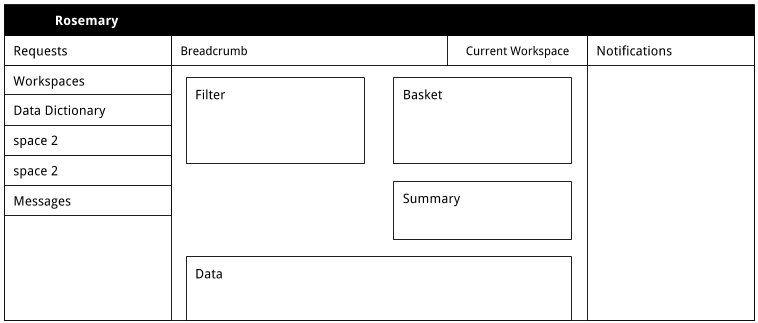
\includegraphics[width=1.0\linewidth]{images/evaluation-layout}
	\caption{
		ireframe representation of the UI layout, showing the data management features: filter, view, select.
	}
	\label{fig:wireframe-layout}
\end{figure}

\begin{figure}[hb]
	\centering
	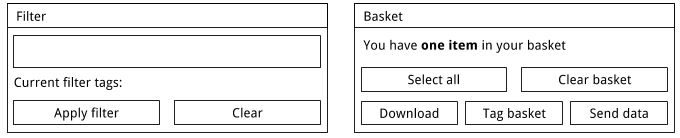
\includegraphics[width=1.0\linewidth]{images/evaluation-basket-layout}
	\caption{
		Wireframe representation of the UI for filter and basket layout, showing the search and select data management tools.
		(Details of the filter and basket blocks in figure \ref{fig:wireframe-layout}).
	}
	\label{fig:wireframe-basket-layout}
\end{figure}